\documentclass{beamer}
%
% Choose how your presentation looks.
%
% For more themes, color themes and font themes, see:
% http://deic.uab.es/~iblanes/beamer_gallery/index_by_theme.html
%
\mode<presentation>
{
  \usetheme{default}      % or try Darmstadt, Madrid, Warsaw, ...
  \usecolortheme{default} % or try albatross, beaver, crane, ...
  \usefonttheme{default}  % or try serif, structurebold, ...
  \setbeamertemplate{navigation symbols}{}
  \setbeamertemplate{caption}[numbered]
} 

\usepackage[english]{babel}
\usepackage[utf8x]{inputenc}
\usepackage{xcolor}

\title{Discovering Barley Intake Biomarkers in Urine by UPLC-MS Based Untargeted Metabolomics}
\subtitle{Project outside coursescope, MSc (15 ECTS)}
\author{Tu Hu \newline \tiny{ Supervisor: Gözde Gürdeniz}}
\institute{University of Copenhagen}
\date{9th, Nov}
%% Hi, Henrik and Gözde. Thank you for coming to my exam. I'll present my project to you.
%% The topic is Discovering Barley Intake Biomarkers in Urine by UPLC-MS Based Untargeted Metabolomics. My supervisor is Gözde. 


\begin{document}

\begin{frame}
  \titlepage
  \tiny{CC-BY}\\
  \tiny{@GitHub/tuhulab/bfi-wholegrain/presentation}
\end{frame}

%%
\begin{frame}{Outline}
  \tableofcontents
\end{frame}
%% This is the outline of my presentation.
%% First, I'll first introduce the Background (how the intervention was performed and how the samples were collected)
%% Then, I'll present why we research on barley, why we need to research barley's intake biomarker? What is the societal and scientific importance? and the general workflow for untargeted metabolomics methods for barley intake biomarkers discovery.
%% Then, I'll shortly introduce materials & methods. just some key points.
%% My presentation today will emphasize on results and comclusions.
%% In the end, I'll present perspectives, what i'm going to do in next step.

\section{Background}
 \begin{frame}{Background}
 \begin{figure}[h]
    \centering
    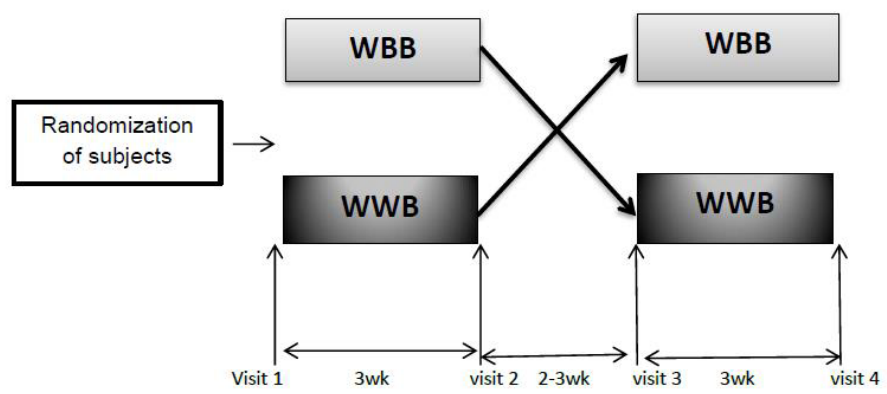
\includegraphics[scale=0.3]{images/studes.PNG}
    \caption{Schema of Study Design (WBB=whole barley bread; WWB=whole wheat bread)}
        \label{fig:studes}
\end{figure}

\begin{itemize}
\item randomized cross-over intervention design
\item 2 bread rolls/day during intervention period
\item 14 healthy volunteers (6 men, 8 women)
\item blood \& urine samples collected each visit
\item Conclusion: No significant changes of CVD risk factors and other health statue factors (before \& after intervention; after barley \& wheat)
\end{itemize}
 \end{frame}
 %% So, first, background. This study was actually based on a previous master thesis in 2016. A randomized cross-over intervention study was designed. During intervention period, the volunteers consumed 2 bread rolls each day.
 %% The conclusion was there's no significant changes of these factors (before & after intervention : the change is not significant) (barley intervention and wheat intervention no significant changes)
 

% P1
\section{Introduction}
\subsection{Barley: from farm to table}
\begin{frame}{Barley: from farm to table}

\begin{columns}[T]
\column{0.5\textwidth}
\textbf{Barley in the farm}
\begin{itemize}
\item \textbf{4th} most produced cereal grains (maize, rice, wheat, \textbf{barley})
\item 143 million tones in 2016
\item Widely adapted species (drought, cold and salt tolerant) - food security
\end{itemize}
 
\column{0.5\textwidth}
\textbf{Barley on the table}
\begin{itemize}
\item 1/3 for malting and brewing (beer)
\item 2\%  for direct food use
\item Majorly for animal's feed
\newline
\item Rough mouthfeel, texture
\item No systematic breeding
\item No quality/ usage standard
\end{itemize}
\end{columns}

\vskip 0.3cm

\begin{block}{Facts (2016)\footnote{statistics from FAO}}
EU produced \textbf{63\%} barley.\\Turkey (\textbf{9th}) \& Denmark (\textbf{11th})  \& China (\textbf{19th}) ranked by barley production 
\end{block}

\end{frame}
%% Let's move backward a little bit. Why barley was chosen as the research object?
%% Let's look at barley in the farm: barley is the 4th most produced cereal grains world-widely (first is maize, then comes rice, wheat, then barley). In 2016, 143 million tones barley was produced. 
%% And barley is very widely adapted species. It can tolerate drought, cold and salt.
%% However, if we look at barley on the table. 1/3 was used for malting and brewing (mostly for beer). Only 2% barley was directly consumed as food. And barley is major consumed by animals (cows, pigs).
%% Barley's status on the table is incompatable with its in the farm. 

\begin{frame}{Barley production}
\begin{figure}[h]
    \centering
    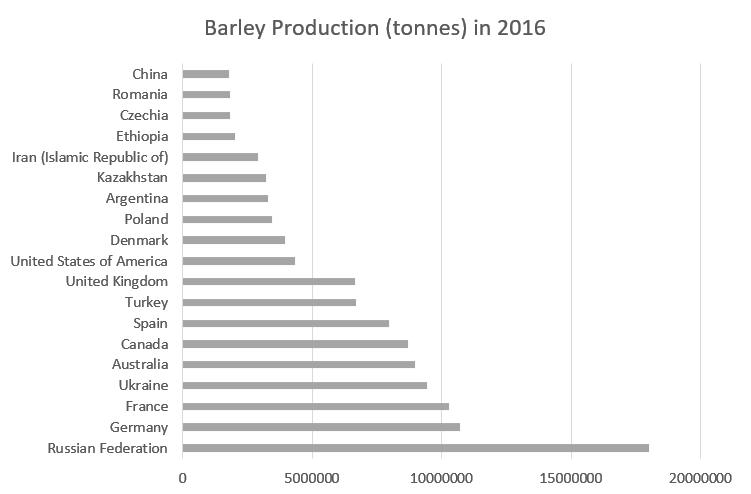
\includegraphics[scale=0.6]{images/barley_production.png}
\end{figure}
\end{frame}

% P2
\subsection{Barley: increasing interest and health benefits}
\begin{frame}{Barley: increasing interest and health benefits}
\begin{columns}[T] 
\column{0.5\textwidth}
\textbf{Increased interest as an healthy ingredient}
\begin{itemize}
\item Customer \& food industry
\newline
\item \textbf{Selling points}
\item Beta-glucan
\item Dietary fiber
\item Whole grain
%% selling points
\end{itemize}
 
\column{0.5\textwidth}
\textbf{Health beneficial effects}
\begin{itemize}
\item \textbf{Beta-glucan} content: 4.6\%
\item capable of reducing cholesterol; regulate blood glucose
\item \textbf{Phytochemicals} (polyphenols, sulfur compounds, lignin and phytic acid)
\item antioxidant activites and  other unknown effects
\end{itemize}
\end{columns}
\vskip 0.3cm

\begin{block}{Conclusions on health benefits}
Controversial. Both positive and negative results were reported.
\textbf{Lack of objective measurement of barey dietary exposure.}
\end{block}
\end{frame}

%P3
\subsection {Biomarkers of Food Intake (BFIs)}
\begin{frame}{Biomarkers of Food Intake (BFIs)}
\textbf{Traditional way to measure dietary exposure}
\begin{itemize}
  \item Self-reported: 24-h dietary recalls, food-frequency questionnarires
  \item subjective (recall bias, difficult to assess portion size ... )
  \item alcohol or tobacco consumption (affected by cultural or societal attitute )
  \item `pressurized' to pretend a healthy diet
\end{itemize}

\textbf{Biomarkers of Food Intake}
\begin{itemize}
  \item Objective
  \item Precise, detailed, informative, dynamics
  \item Metabolic \& signaling pathway
\end{itemize}
\end{frame}

%%
\begin{frame}{Alkylresorcinols: biomarkers of whole grain cereal intake}

\textbf{Current status}
\begin{itemize}
	\item Widely reported and validated biomarker for whole grain cereals (Table)
	\item Detected both in urine and plasma
\end{itemize}

\textbf{Limitations}
\begin{itemize}
	\item Taking account of all whole grain cereals. 
	\item Not specific to individual grain type (wheat, rye, oats, barley...)
	\item No barley biomarkers reported
\end{itemize}
\end{frame}

%%
\subsection{Whole Grain Cereal Intake Biomarkers}
\begin{frame}{Alkylresorcinols}
\begin{figure}[h]
    \centering
    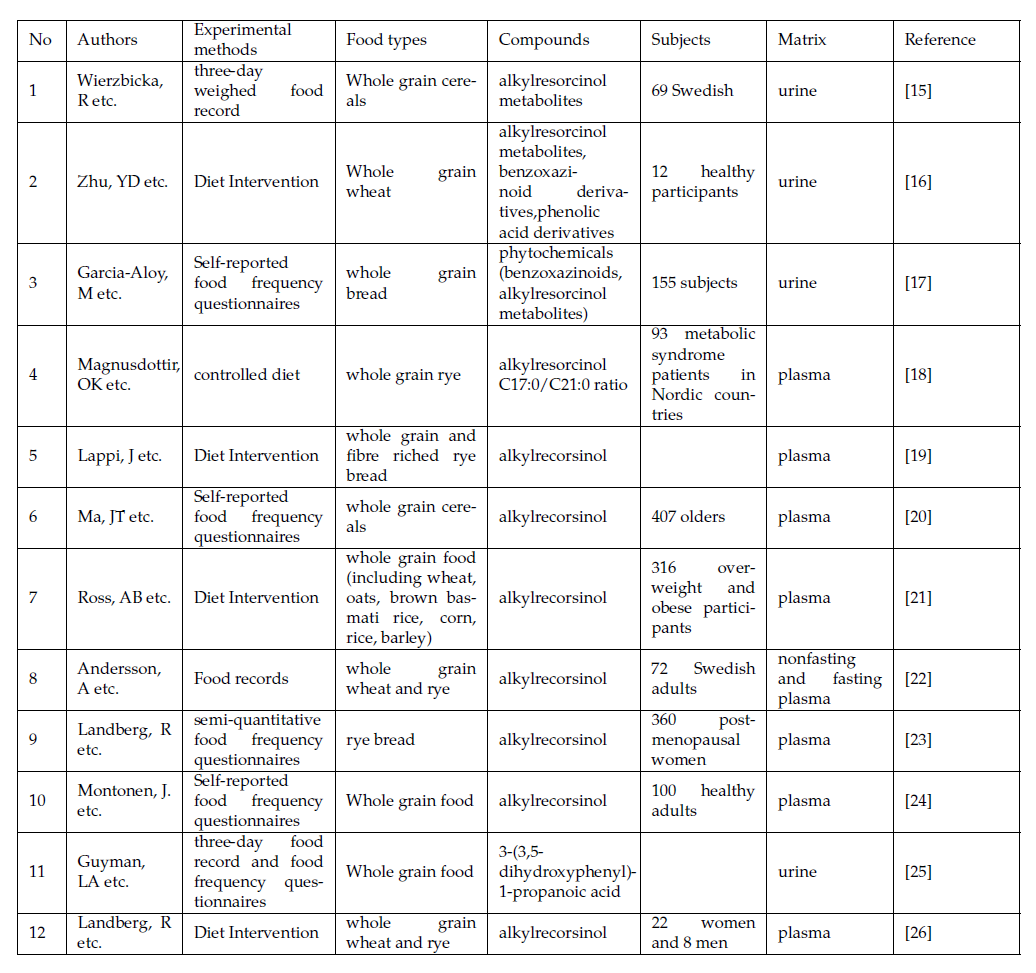
\includegraphics[scale=0.32]{images/alkylresorcinols.png}
\end{figure}
\end{frame}

%%
\subsection{Workflow of BFIs discovery by Untargeted Metabolomoics}
\begin{frame}{Workflow of BFIs discovery by Untargeted Metabolomoics}
\begin{itemize}
	\item Metabolome profiling (\textbf{LC-MS}, GC-MS, 1-NMR)
	\item Data preprocess
	\item Data analysis 
	\item<1-> \textbf{Compound identification}
		\begin{itemize}
			\item Most difficult part in all areas of metabolomics study
			\item \textbf{Expert opinions} (1st Copenhagen Clinical Metabolomics Conference) 
		\end {itemize}
	\item Validation
\end{itemize}
\end{frame}

\begin{frame}{Compound identification: expert opinions}
\begin{itemize}
	\item \textbf{Improvement of analytical instruments for metabolome profiling:}\\ 
	e.g TIMF-PASEF (ion mobility, rt, m/z and intensities)
	\item \textbf{Bioinformatics, database and data sharing:}\\
	MS/MS prediction, HMDB, GNPS, molecular networking
	\item \textbf{Deepening the understanding of biological aspect of metabolism}
	\item \textbf{'Correctly' identify the identifiable compounds:}\\
	strict experimental conditions, in-house database (lipidomics)
	
\end{itemize}
\end{frame}

\section{Materials \& Methods}
\subsection{Highlights}
\begin{frame}{Materials \& Methods: highlights}
\begin{itemize}
\item 2 sets of \textbf{LC-MS} system were used; 2 \textbf{LC methods} were used (7 min, 10 min)
\item 2 fractions of whole grain barley powder: \textbf{bran (brownish) from outlayer}, \textbf{endosperm (white) from inner}
\end{itemize}
\end {frame}

\section{Results}
%%
\subsection{LC-MS analysis of Whole Grain Barley}
\begin{frame}{LC-MS analysis of Whole Grain Barley}
\begin{figure}[h]
    \centering
    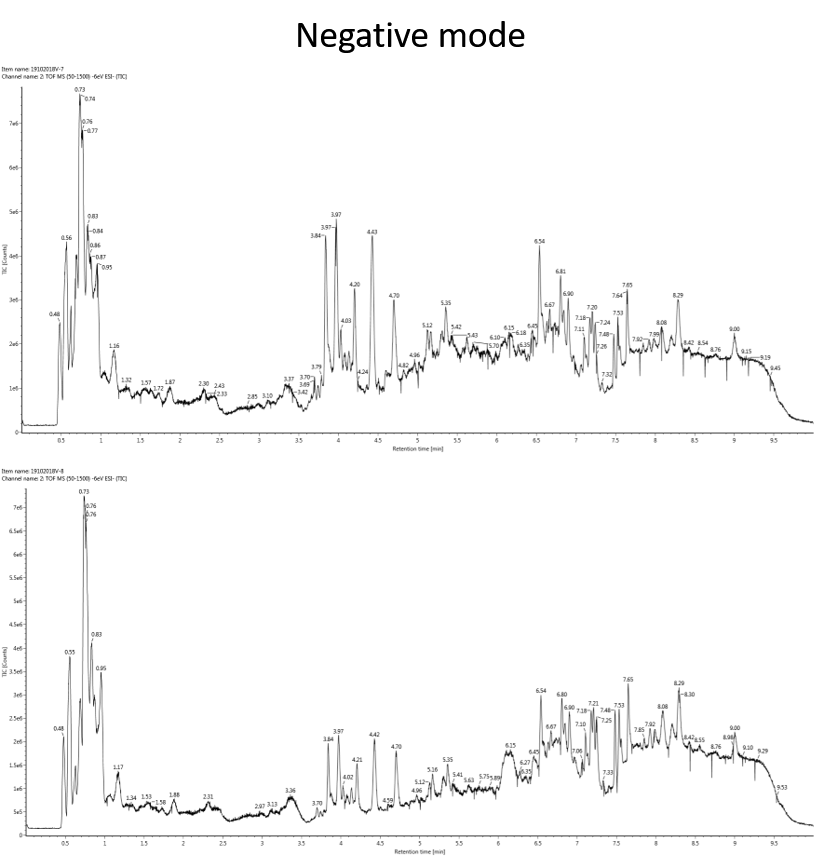
\includegraphics[scale=0.25]{images/chromatogram_barley_neg.png}
\end{figure}
\small{
\begin{block}{Bran (\textbf{top}) vs Endosperm (\textbf{bottom}) powder chromatograms} Same pattern. Retention time shift within 0.02 min. Higher intensities of \textbf{bran} powder in some peaks resulted from (1) experimental error (2) `whole grain' dissolved more in ethanol/water.
\end{block}}
\end{frame}
%% As I mentioned before, bran powder and endosperm powders of barley were analyzed separately.
%% In general, they have the same pattern. RT shift was between 0.02 min. 
%% But, we also observed that, bran powder had higher intensities in some peaks.



%%
\subsection{Data Preprocess }
\begin{frame}{Data Preprocess }
\begin{table}
\centering
\begin{tabular}{c|c}
Mode & Number of feature detected \\\hline
positive & 1719 \\
negative & 3304
\end{tabular}
\end{table}
\begin{block}{Possible reasons for more features were detected in negative mode}
\begin{itemize}
\item Negative mode had better resolving power
\item Metabolites from urine (e.g. glucoronate conjugates) were easier ionized in negative mode.
\end{itemize}
\end{block}
\end{frame}

%%
\subsection{PCA modeling}
\begin{frame}{PCA modeling}
\begin{figure}[h]
    \centering
    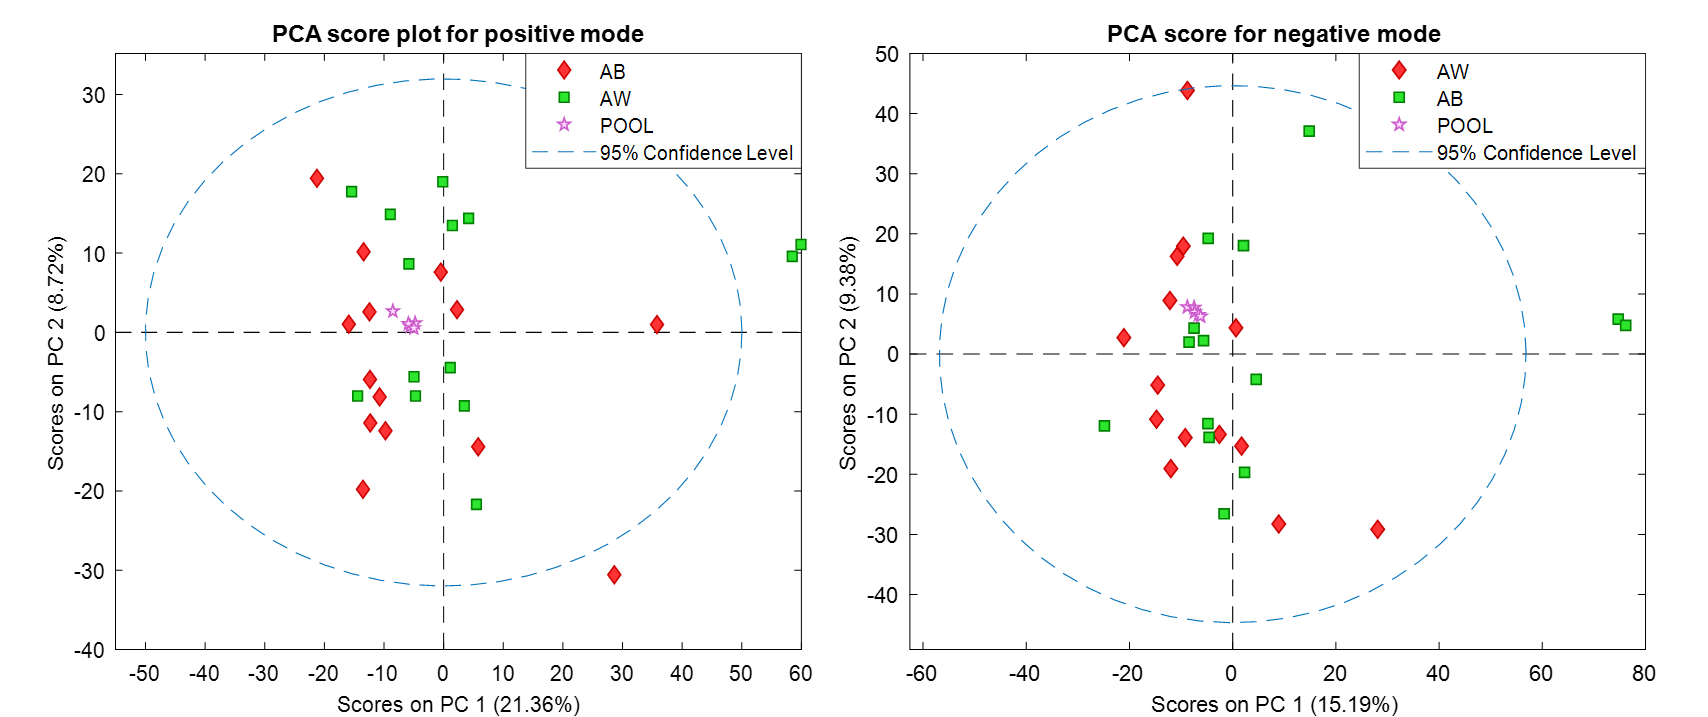
\includegraphics[scale=0.3]{images/pca_score.png}
    \caption{PCA score plot (AW= After Wheat, AB= After Barley, POOL= pooled samples)}
\end{figure}

\begin{itemize}
\item AB \& AW were not separated in score plots
\item POOL located tightly near the center: high quality data
\item Outliers: because of too concentrated urine (high intensities of all variables)

\end{itemize}
\end{frame}

%%
\subsection{PLSDA Modeling and Variable Selections}
\begin{frame}{PLSDA Modeling and Variable Selections}

\begin{table}
\centering
\begin{tabular}{c|c}
Mode & Variables selected (out of) \\\hline
positive & 72 (1719) \\
negative & 86 (3304)
\end{tabular}
\end{table}

\begin{figure}[h]
    \centering
    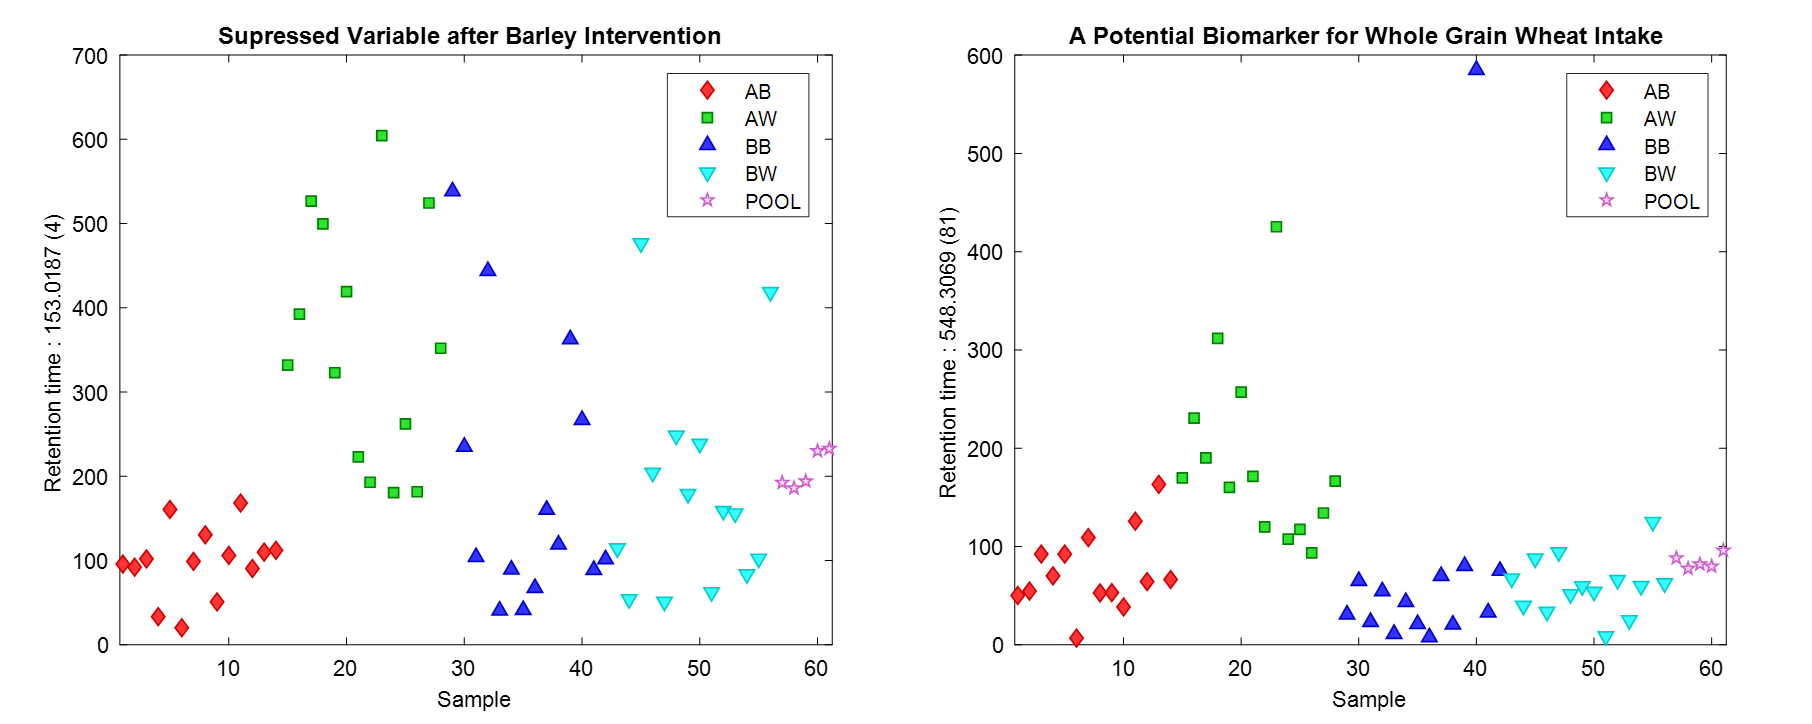
\includegraphics[scale=0.25]{images/marker1.png}
    \caption{Variables Selected by PLSDA modeling but not classified as potential barley intake biomarkers}
    \label{fig:marker1}
\end{figure}
\begin{itemize}
\item (left) Intensities suppressed after barley intake; could be an endogenous metabolite
\item (right) wheat intake biomarker


\end{itemize}
\end{frame}

\begin{frame}{PLSDA Modeling and Variable Selections}

\begin{figure}[H]
    \centering
    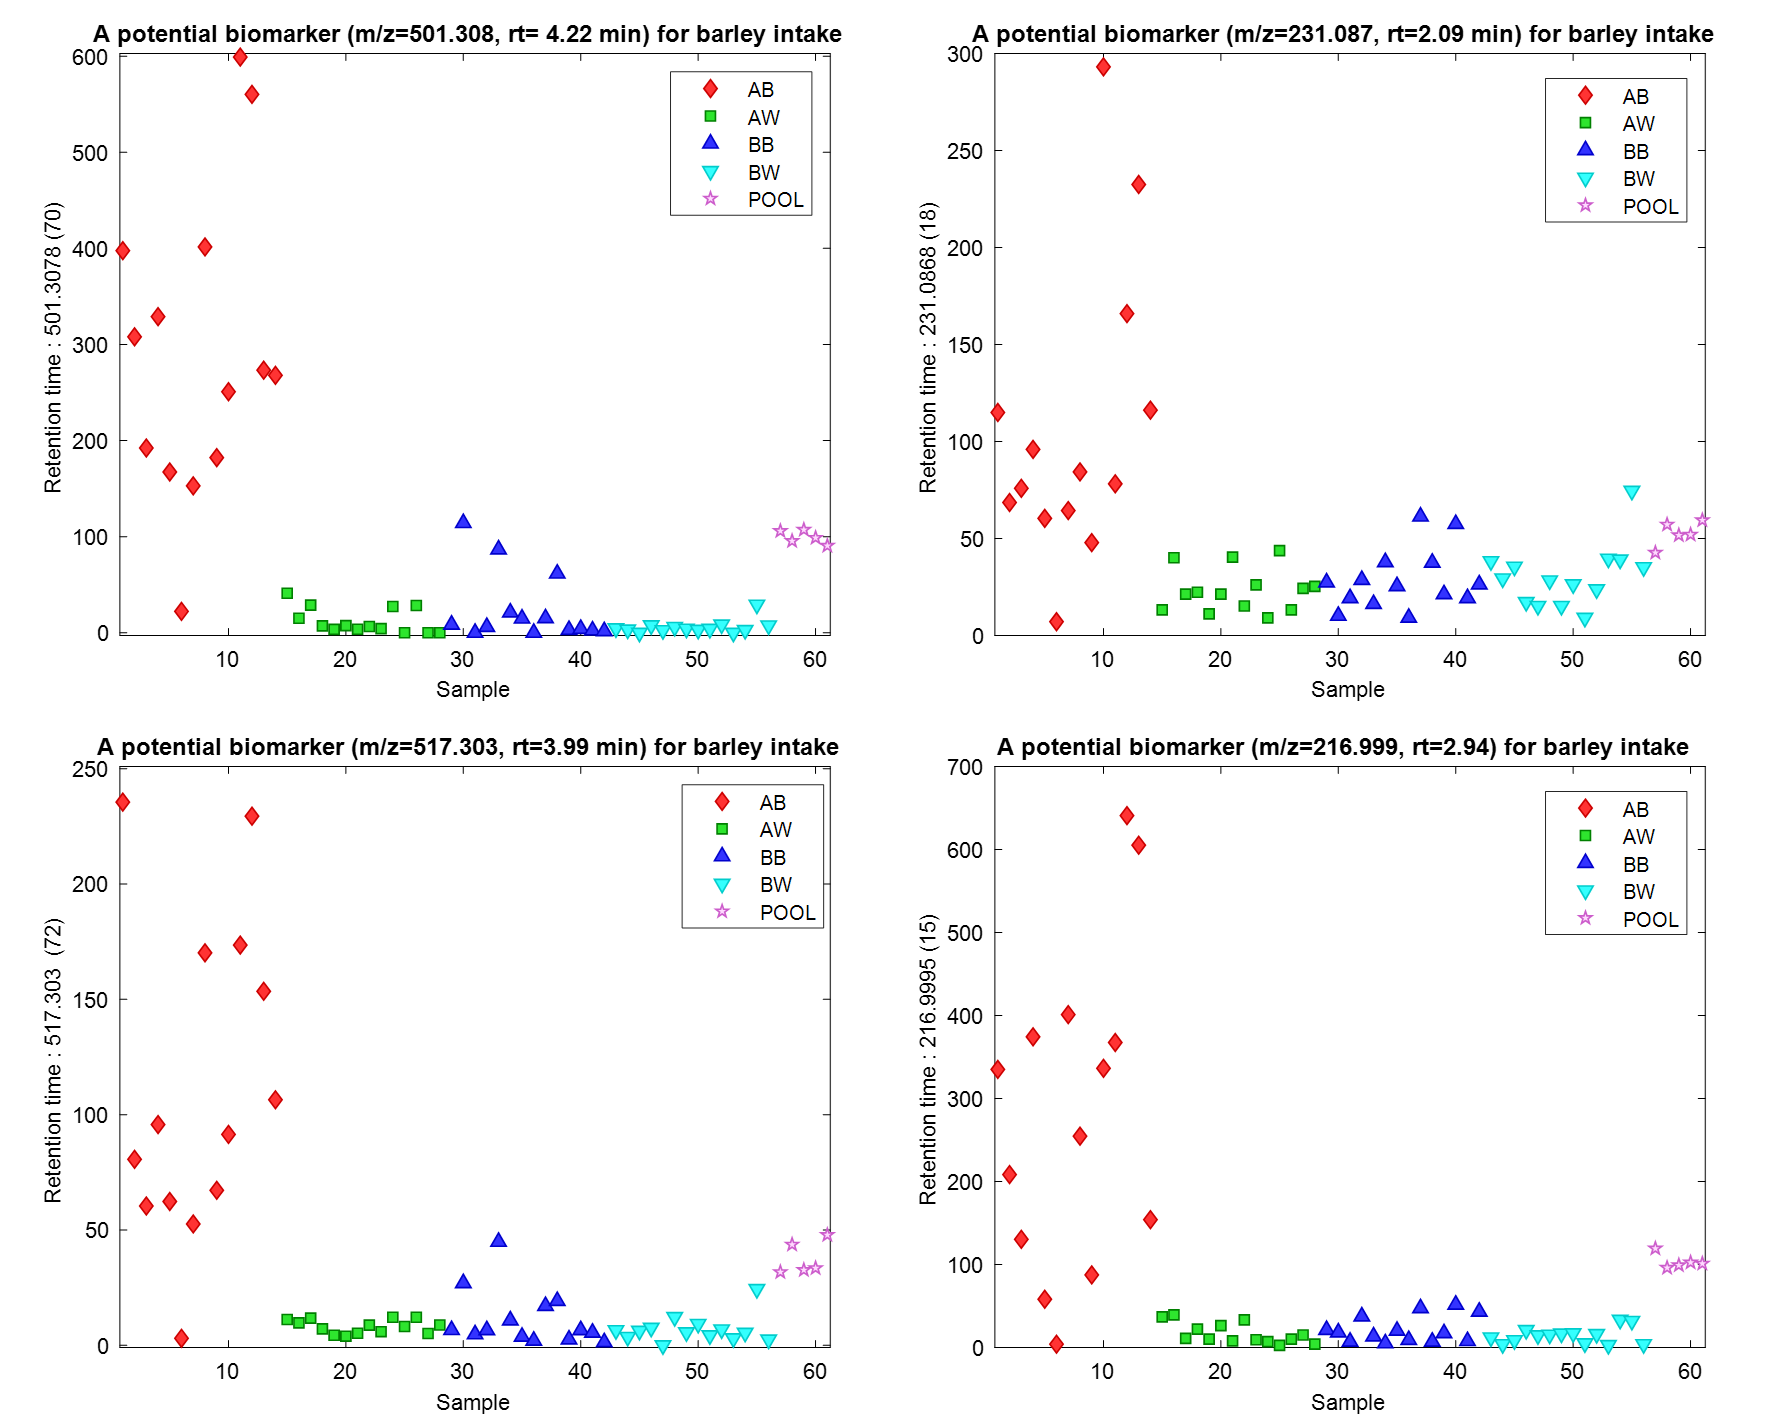
\includegraphics[scale=0.25]{images/barley_marker.png}

    \label{fig:selected}
\end{figure}


\begin{itemize}
\item \textbf{Role of thumb}
\item Nearly no background signals
\item Increased intensities after barley intake
\end{itemize}

\end{frame}

%%
\begin{frame}{PLSDA Modeling and Variable Selections}

\begin{table}
\centering
\begin{tabular}{c|c}
Mode & Potential Biomarkers selected for MS/MS\\\hline
positive & 1 (m/z= 291) \\
negative & 5 (m/z= 517, 501, 775, 216)
\end{tabular}
\end{table}
\end{frame}

%%

%%
\subsection{MS/MS and Identification}
\begin{frame}{MS/MS and Identification: m/z 231.0870 (ESI-)}
\begin{figure}[h]
    \centering
    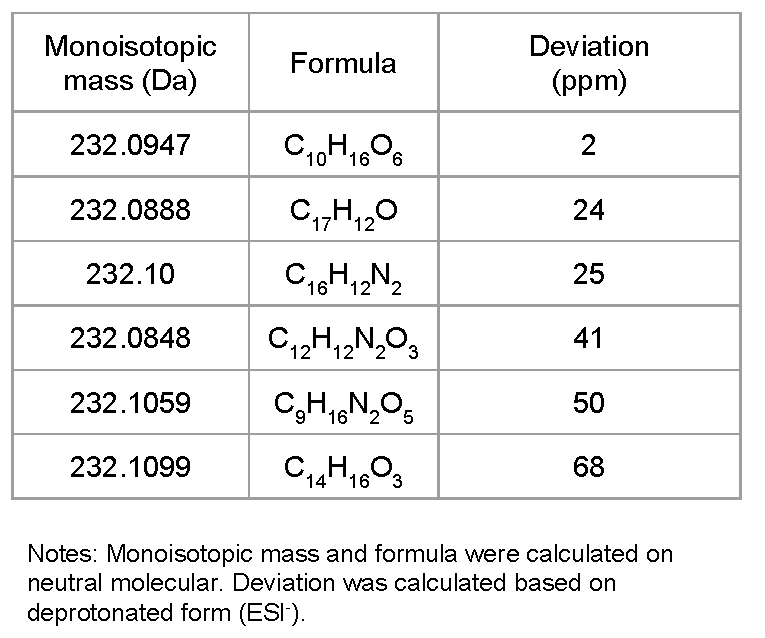
\includegraphics[scale=0.5]{images/231p0870.pdf}
    \caption{Possible formulas of ion m/z 231.0870}
    \label{fig:231p0870}
\end{figure}
\begin{block}{Intensity was too low for MS/MS}
\end{block}
\end{frame}

%%
\begin{frame}{MS/MS and Identification: m/z 775.3401 (ESI-)}

\begin{itemize}
\item Dimer of [C\textsubscript{18}H\textsubscript{28}O\textsubscript{9}-H]\textsuperscript{-} with neutral mass 388.1735

\item Intensity was too low for MS/MS
\end{itemize}
\end{frame}

%%
\begin{frame}{MS/MS and Identification: m/z 216.9995 (ESI-)}

\begin{itemize}
\item Intensity was too low for MS/MS
\item Feasible hints exist in HMDB. Whole grain barley riches in benzoic acid, phenol and polyphenol
\begin{figure}[h!]
    \centering
    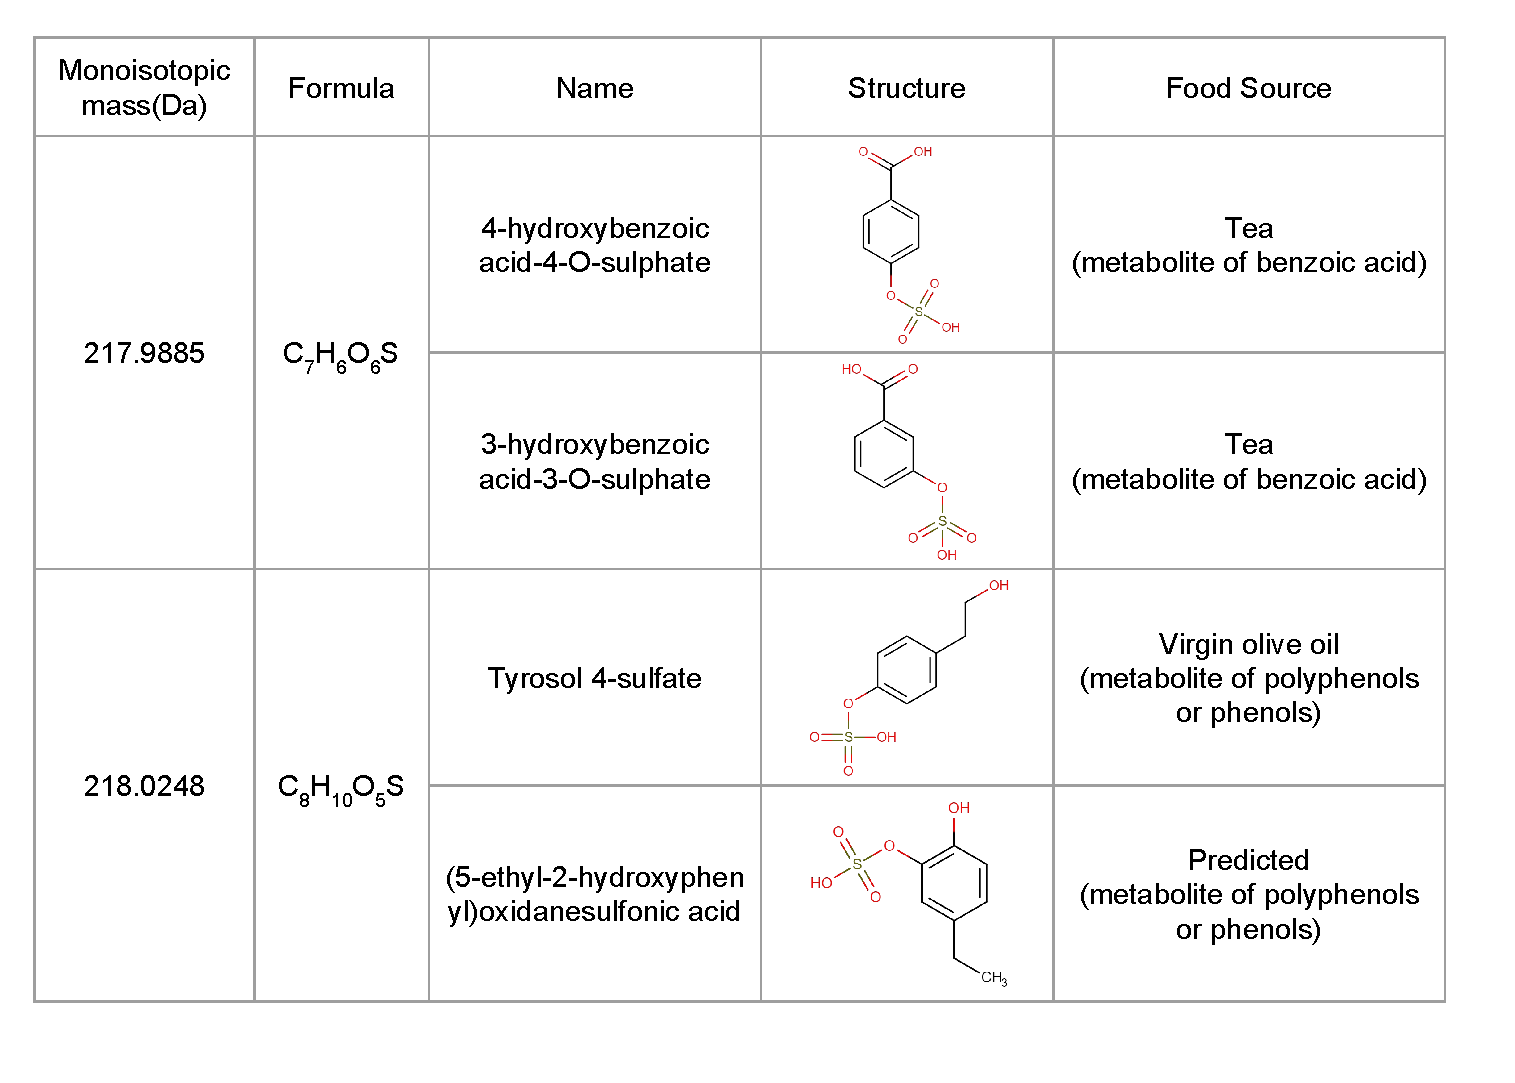
\includegraphics[scale=0.35]{images/216d9995.pdf}

    \label{fig:216p9995}
\end{figure}
\end{itemize}
\end{frame}

%%
\begin{frame}{MS/MS and Identification: m/z 517.3030, 501.3080 (ESI-)}
\begin{itemize}
\item C\textsubscript{30}H\textsubscript{46}O\textsubscript{7} and C\textsubscript{30}H\textsubscript{46}O\textsubscript{6}
\item Glucuronide conjugates of barley metabolites
\item Common lost of glucuronidyl group (-176)
\item Unconjugated ions detected (NOT identifiable)
\item Low-mass region interfered by 2nd fragmentation of glucuronyl group
\end{itemize}
\begin{figure}[h]
    \centering
    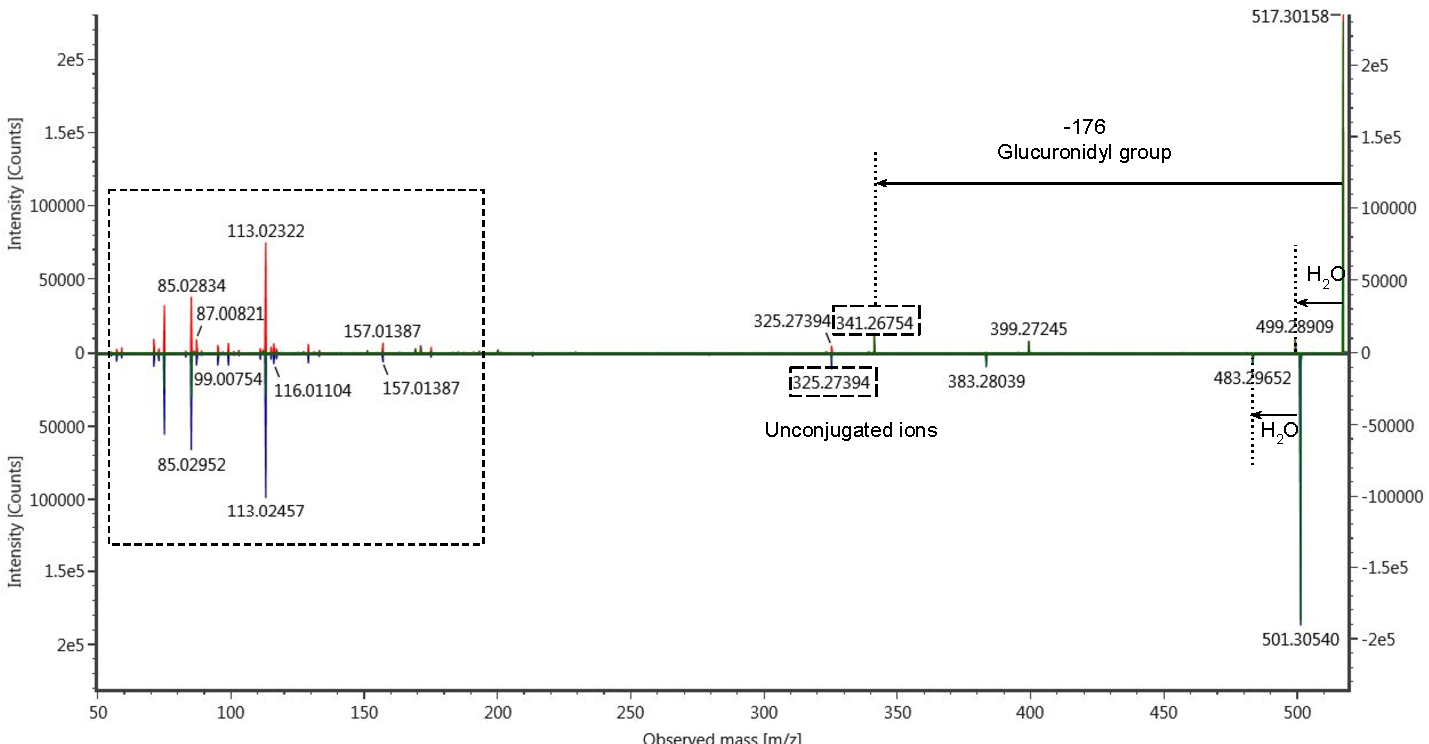
\includegraphics[scale=0.38]{images/501517compare.pdf}

    \label{fig:501517compare}
\end{figure}
\end{frame}
%%
\begin{frame}{MS/MS and Identification: m/z 517.3030, 501.3080 (ESI-)}
\begin{figure}[h!]
    \centering
    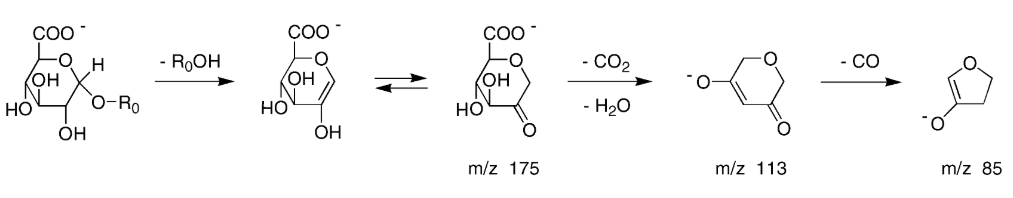
\includegraphics[scale=0.40]{images/gluco_frag.PNG}
    \caption{Secondary fragmentation of the glycuronyl moiety in negative-ion MS/MS spectra of glucuronide conjugates.}
    \label{fig:gluco_frag.PNG}
\end{figure}
\end{frame}

%%
\begin{frame}{MS/MS and Identification: m/z 291.2683 (ESI+)}
\begin{itemize}
\item Originated from `whole grain part' (bran) 
\item Same structure detected in urine and barley samples
\item Annotated as phytosterol or its derivative or its in-source fragment
\end{itemize}
\end{frame}
%%
\begin{frame}{MS/MS and Identification: m/z 291.2683 (ESI+)}
\begin{block} {Originated from `whole grain part' (bran) }
\begin{itemize}
\item \textbf{Intensity higher in bran than endosperm}
\item MS/MS showed same structure
\end{itemize}
\begin{figure}[H]
    \centering
    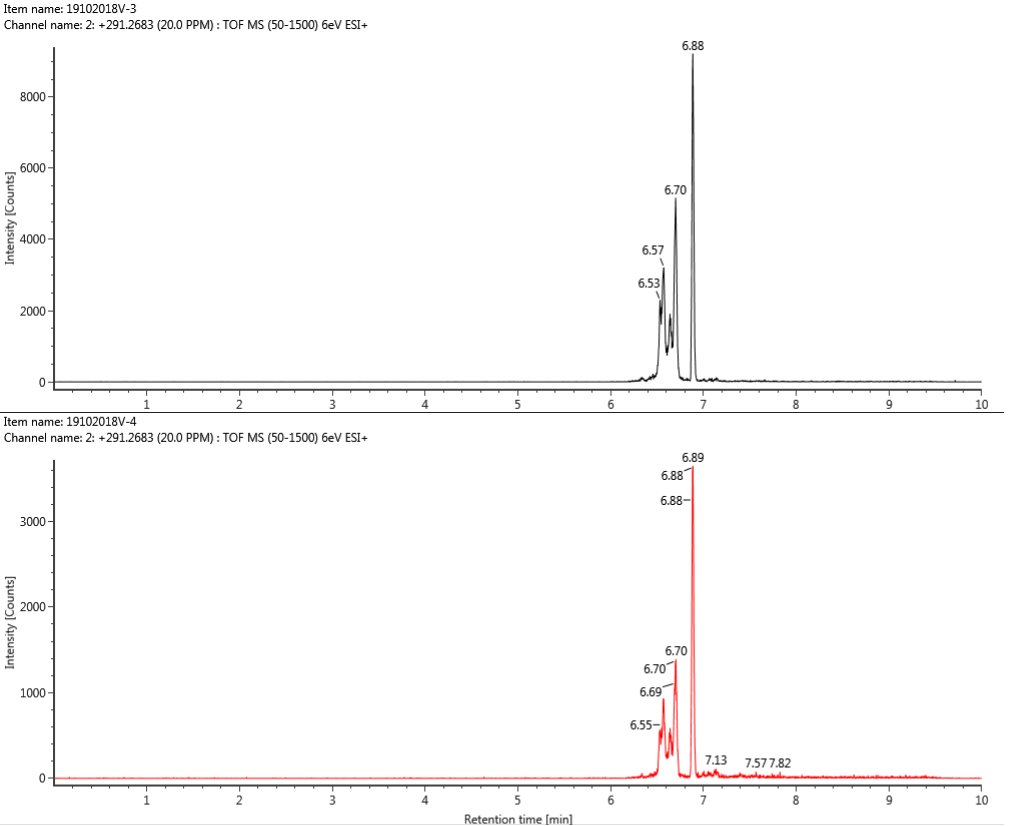
\includegraphics[scale=0.25]{images/291pos(p1,p2).png}
    \caption{Chromatograms of ion(m/z=291.2683) in bran powder and endosperm powder. Top (bran); bottom (endosperm).}
    \label{fig:291_barley}
\end{figure}
\end{block}
\end{frame}

%%
\begin{frame}{MS/MS and Identification: m/z 291.2683 (ESI+)}
\begin{block} {Same structure detected in urine and barley samples}
\begin{itemize}
\item Similar retention time (min) (barley:6.88, urine:6.71)
\item Same MS/MS pattern
\end{itemize}
\begin{figure}[H]
    \centering
    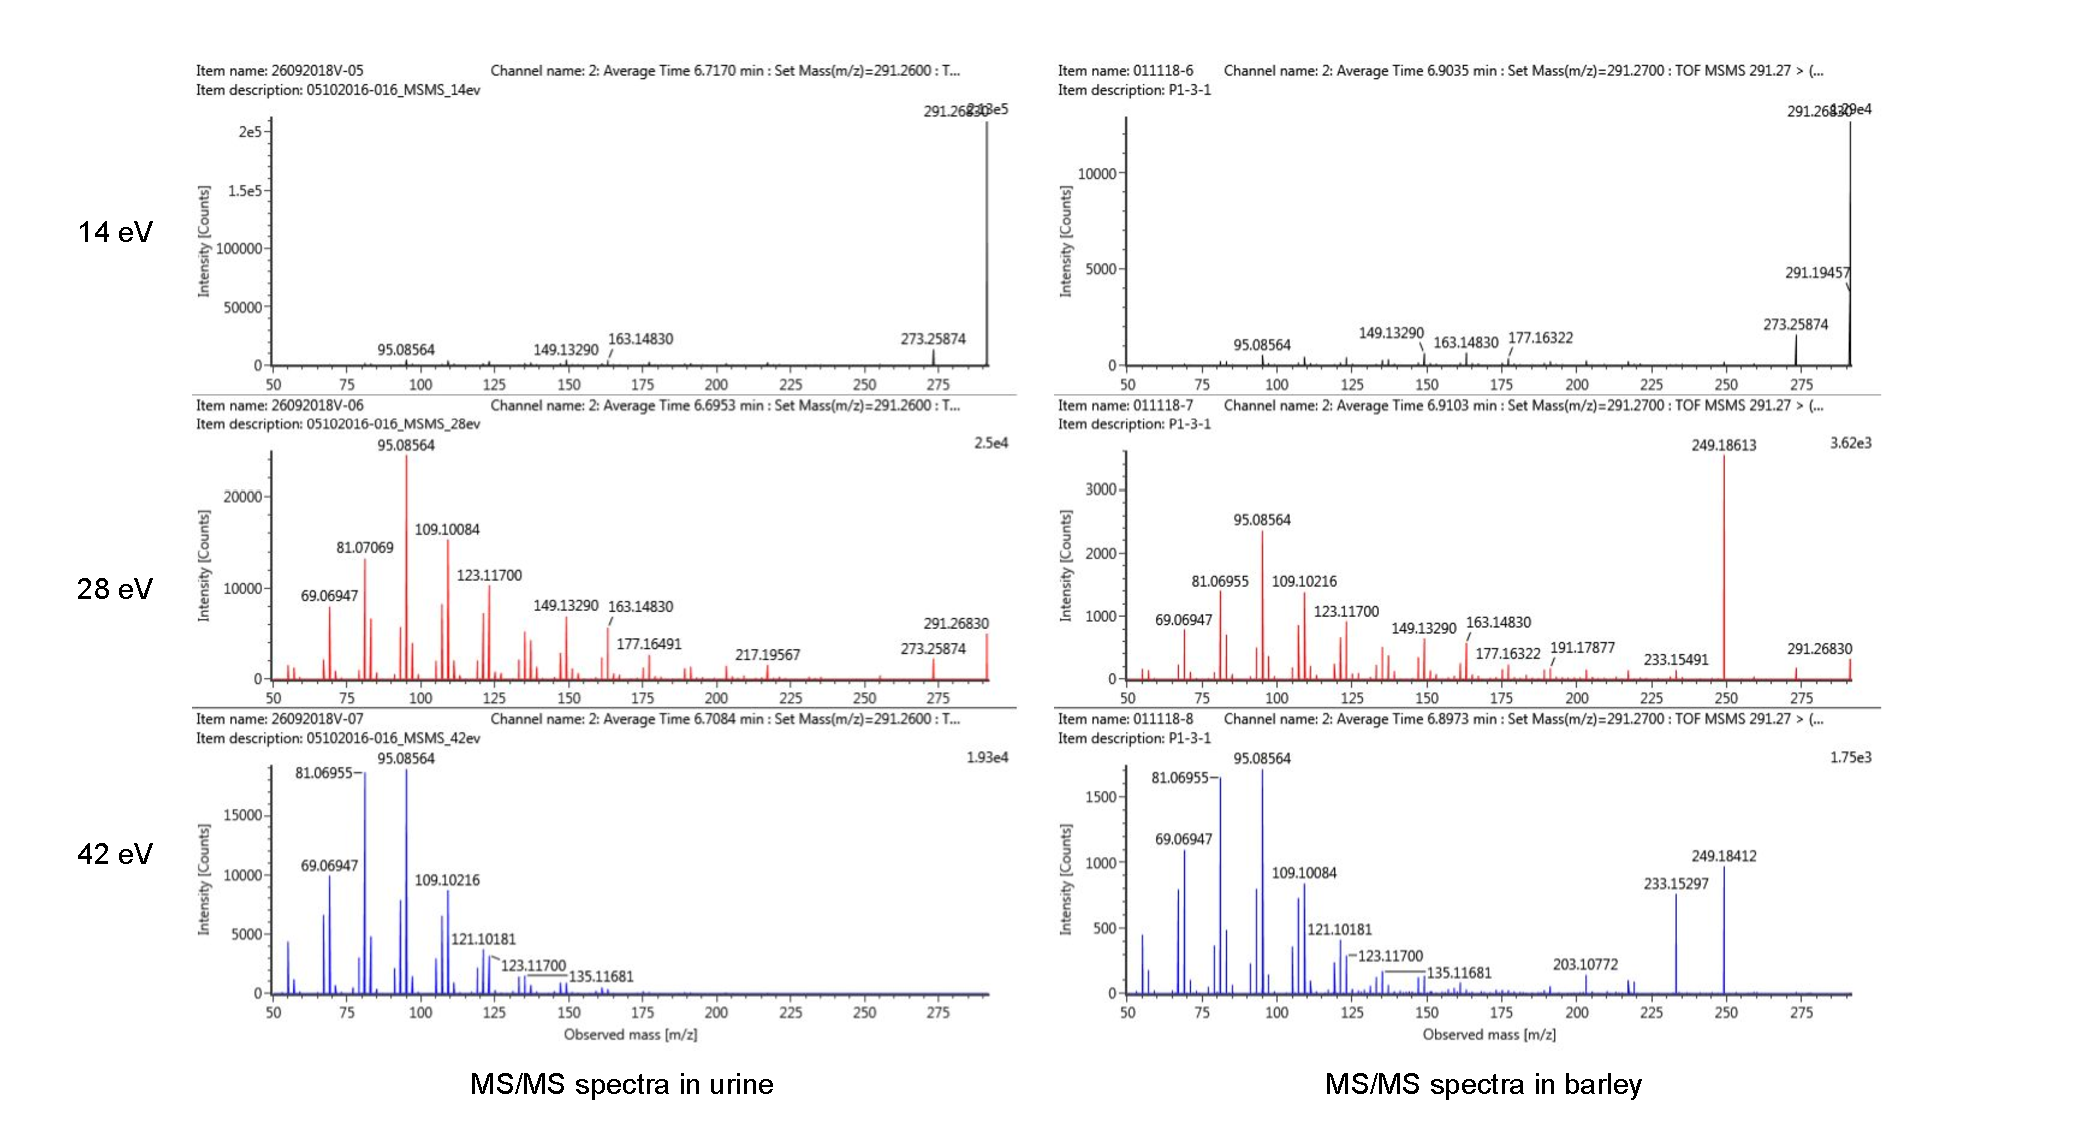
\includegraphics[scale=0.25]{images/ION291.pdf}
    \caption{MS/MS spectra of ion (m/z=291.2683) in urine and barley sample with different collision energies}
    \label{fig:MSMSION291}
\end{figure}
\end{block}
\end{frame}
%%
\begin{frame}{MS/MS and Identification: m/z 291.2683 (ESI+)}
\begin{block} {Putatively annotated as sterol (or its derivative)}
\begin{itemize}
\item \textbf{MS/MS pattern} matches common sterols
\item However, too low mass compared with common sterols
\end{itemize}
\begin{figure}[H]
    \centering
    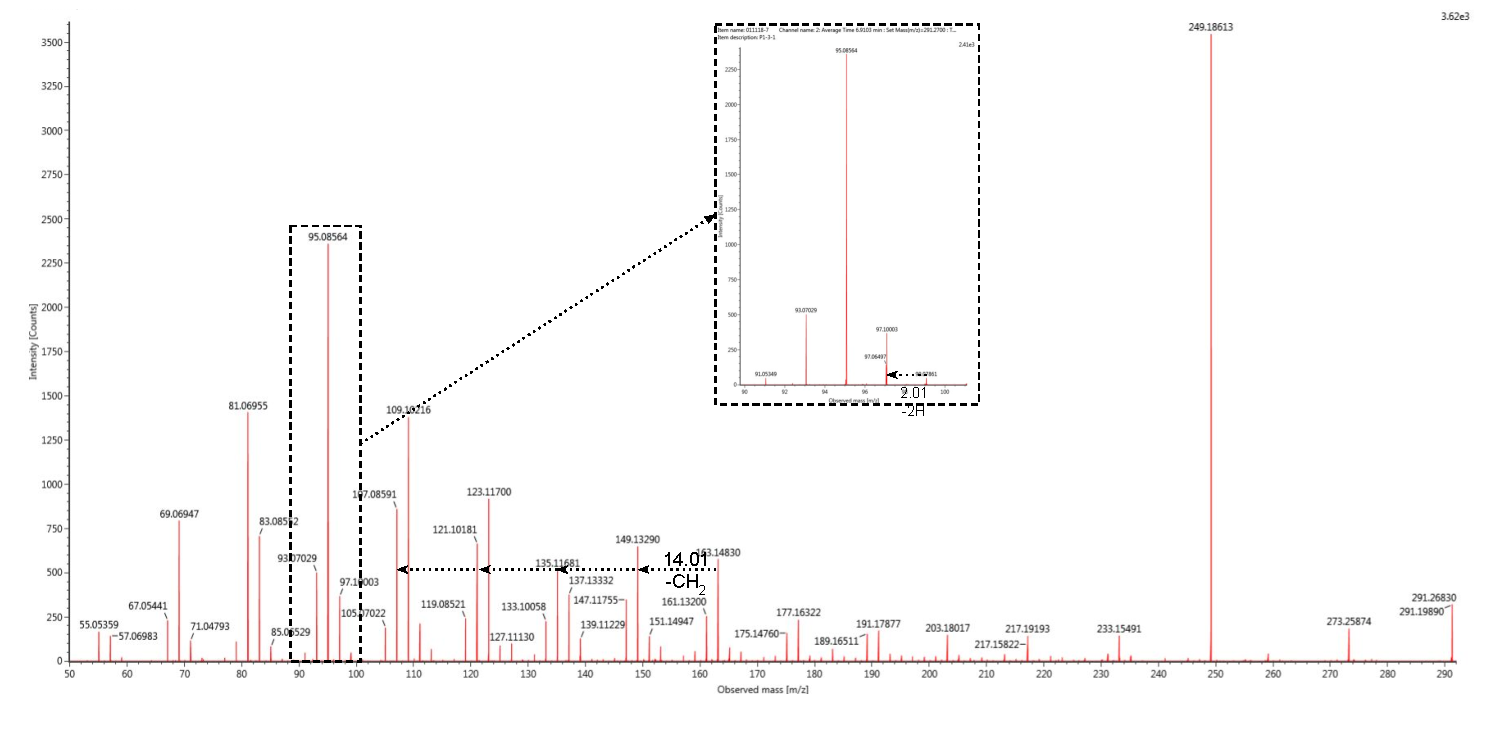
\includegraphics[scale=0.35]{images/Annotation-291.pdf}
    \caption{MS/MS spectra of ion(m/z=291.2683) in barley sample (Collision energy = 24 eV)}
    \label{fig:291_barley1}
\end{figure}
\end{block}
\end{frame}
%%
\begin{frame}{MS/MS and Identification: m/z 291.2683 (ESI+)}
\begin{block} {Putatively annotated as sterol (or its derivative)}
\begin{itemize}
\item MS/MS pattern matches \textbf{common sterols}
\end{itemize}
\end{block}
\begin{figure}[H]
    \centering
    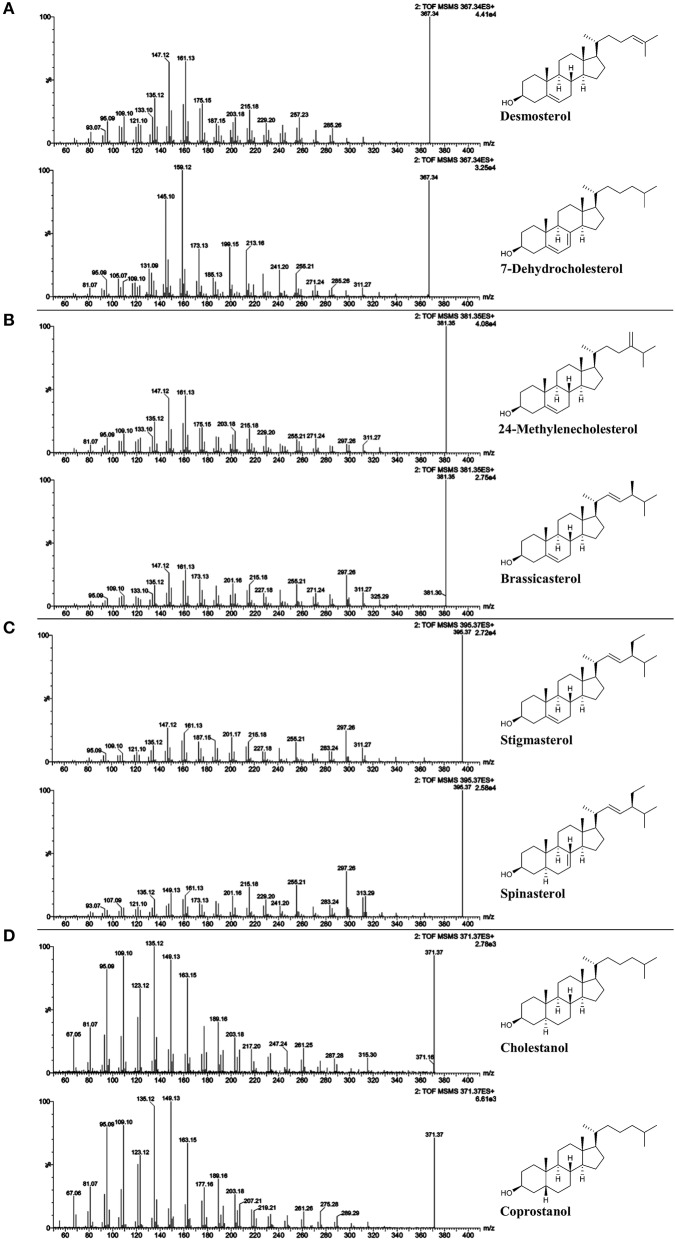
\includegraphics[scale=0.6]{images/sterolmsms.jpg}
    \label{fig:sterolmsms}
\end{figure}

\end{frame}
%%
\begin{frame}{MS/MS and Identification: m/z 291.2683 (ESI+)}
\begin{block} {Putatively annotated as sterol (or its derivative)}
\begin{itemize}
\item MS/MS pattern matches common sterols
\item However, too low mass compared with \textbf{common sterols}
\end{itemize}
\begin{figure}[H]
    \centering
    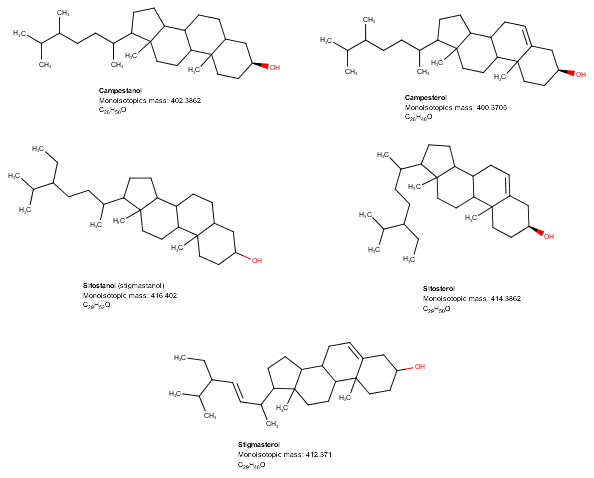
\includegraphics[scale=0.27]{images/5sterols_combined.png}
    \caption{Major sterols in barley)}
    \label{fig:5sterol}
\end{figure}
\end{block}
\end{frame}
%%

\begin{frame}{MS/MS and Identification: m/z 291.2683 (ESI+)}
\begin{block} {Putatively annotated as sterol (or its derivative)}
\begin{itemize}
\item MS/MS pattern matches common sterols
\item However, too low mass compared with \textbf{common sterols}
\end{itemize}

\begin{figure}[H]
    \centering
    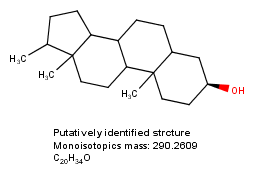
\includegraphics[scale=0.5]{images/possiblesterol.png}
    \caption{Putatively identified structure}
    \label{fig:putativesterol}
\end{figure}

\end{block}
\end{frame}
%%
\section{Conclusions \& Discussions}
\begin{frame}{Conclusions \& Discussions}
\begin{figure}[H]
    \centering
    
\includegraphics[scale=0.6]{images/idsummarybarley.PNG}
    \caption{Identification summary}
    \label{fig:idsummary}
\end{figure}
\end{frame}
%%

\begin{frame}{Conclusions \& Discussions}

\begin{block} {Metabolome of phytochemicals could indicate plant-source food intake}
\begin{itemize}
\item Annotated compounds appeared to be phytochemicals (and their metabolites).
\item Identification, quantification and database of phytochemicals NOT mature.
\item More phytochemicals could be studied.
\end{itemize}
\end{block}

\begin{block} {Phytochemicals}
\begin{itemize}
\item a general term for chemicals produced by plants
\item functions for human not clarified
\item varied a lot of between species
\item metabolome of plants, controlled by plants' gene expression
\end{itemize}
\end{block}
\end{frame}
%%
\section{Perspectives (Next step)}
\begin{frame} {Perspectives (Next step/6 month)}

\begin{itemize}
\item \color{gray} Barley - Urine/\color{black}Plasma  ;  Wheat - Urine/Plasma
\item Get hints from other dataset (Mediterranean, New Nordic)
\item More perspectives
	\begin {itemize}
		\item \textbf{Foodomics (Foodome)}
		\item New concept initiated from 2009; even more `emerging' than metabolomics
		\item Omics methods for food 
		\item We have a lot of data of food (barley and wheat's MS profile)
		\item \textbf{Be critical}
	\end {itemize}
\begin{figure}[H]
    \centering
    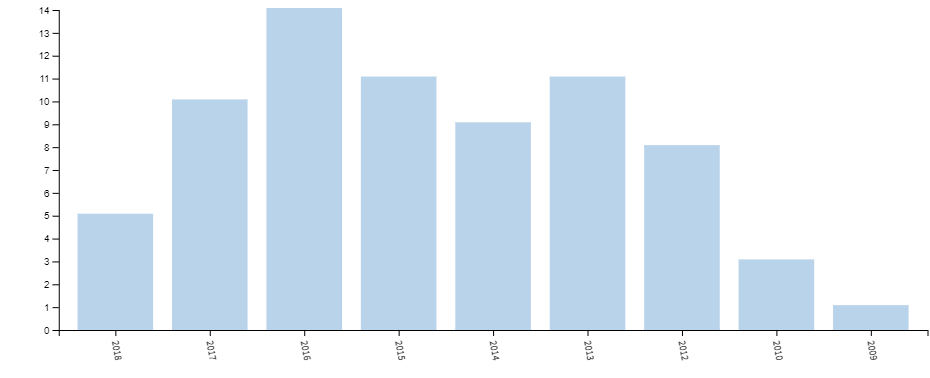
\includegraphics[scale=0.27]{images/foodomics.jpg}
    \caption{Articles with `foodomics' and `foodome' as topic in Web of Science}
\end{figure}
\end{itemize}
\end{frame}
%%
\begin{frame} {Perspectives (Next step/6 month)}

	\begin {itemize}
		\item \textbf{Bioinformatics Tools (open source)}
		\item MetaboDiff (comparative metabolomics) - R package
		\item MAIT (Metabolite Automatic Identification Toolkit) - R package
	\end {itemize}
\end{frame}
%%



\section{Acknowledgements}
\begin{frame}{Acknowledgements}
My supervisor Gözde.\\ Henrik, Lars \\ All fellows and technicians\\
\end{frame}

\end{document}
